\section{Modeling Strategy}
\label{sec:modeling:strategy}
To create a model for the architecture, the chosen strategy was to base it on
the principles explained in Chapter~\ref{cha:cache_coherence}. In effect, the
architecture is reduced to elements directly relevant to cache coherence. The
assumption is that any user requiring more detail on (or the addition of) a
specific component's model can either adapt it from another UPPAAL
representation of architecture (such as the ones described in
Chapter~\ref{cha:analyzing_rel_work}), or port the cache coherence mechanisms
modeled here to that other model. The coherence protocol to be modeled is
chosen outside of the UPPAAL model, using CoProSwi, a Java program I made in
order to make protocol switching trivial (see
Figure~\ref{fig:second_intro:coproswi}). This tool is explained in more details
in Section~\ref{sec:protocol_switching}.

\begin{figure}[hbt!]
\begin{center}
\begin{tikzpicture}[
  font=\sffamily,
  every matrix/.style={ampersand replacement=\&,column sep=2.5cm,row sep=1cm},
  source/.style={draw,thick,rounded corners,fill=yellow!20,inner sep=.3cm},
  process/.style={draw,thick,circle,fill=blue!20},
  sink/.style={source,fill=green!20},
  datastore/.style={draw,very thick,shape=datastore,inner sep=.3cm},
  dots/.style={gray,scale=2},
  to/.style={->,>=stealth',shorten >=1pt,semithick,font=\sffamily\footnotesize},
  every node/.style={align=center}]

  % Position the nodes using a matrix layout
  \matrix{
   \&
    \node[datastore] (cacheprotocol) {%
         \begin{tabular}{@{}c@{}}
            Cache Coherence\\ Protocol B
         \end{tabular}
         };
      \&
   \\
    \node[datastore] (architecture) {Model with Protocol A};
      \&
      \node[source] (benchmarking) {CoProSwi};
      \&
    \node[datastore] (cacheperformance) {Model with Protocol B};
      \\
  };

  % Draw the arrows between the nodes and label them.
  \draw[to] (architecture) to (benchmarking);
  \draw[to] (cacheprotocol) to (benchmarking);

  \draw[to] (benchmarking) to (cacheperformance);
\end{tikzpicture}

\end{center}
\caption{Co(herence) Pro(tocol) Swi(tcher) utility}
\label{fig:second_intro:coproswi}
\end{figure}

Each component has its own automaton. These automata are designed around the
synchronizations they perform with other automata. As a result, automaton
transitions are mainly present for the purposes of synchronizing, with coherence
behaviors being modeled solely using the C-like UPPAAL language (and thus not
directly visible on the automata). This results in smaller, more readable
automata.

\begin{figure}[hbt!]
\begin{center}
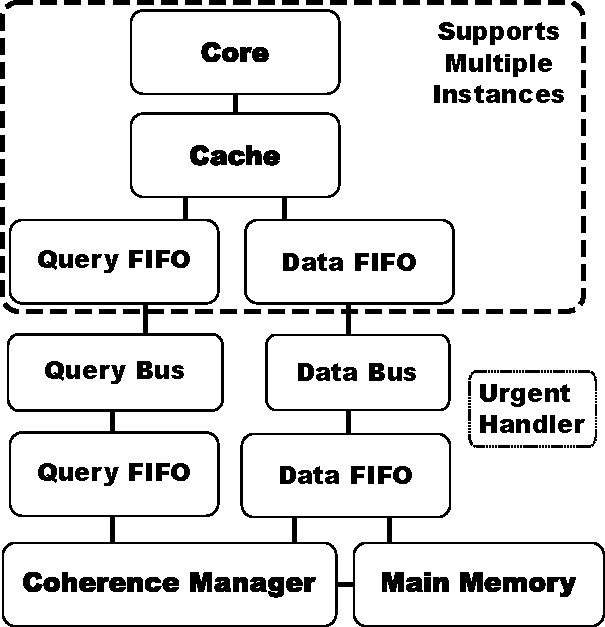
\includegraphics[width=0.5\textwidth]{\chapterdirectory/figure/model_overview.pdf}
\end{center}
\caption{Overview of the Model's Automata}
\label{fig:UPPAAL:automata_overview}
\end{figure}

Figure~\ref{fig:UPPAAL:automata_overview} shows all the automata defined in the
model. Compared to the archetype target architecture presented in
Chapter~\ref{cha:second_intro}, the differences are minor. Indeed, the
\textit{split-transaction interconnect} has been split into its two composing
parts: a \textit{query bus} and a \textit{data bus}. Additionally, a
\textit{data FIFO} automaton has been added, which is shared by the coherence
manager and the main memory. Lastly, an \textit{Urgent Handler} automaton is
present. It does not correspond to any component, but is simply here as an
utility for \texttt{urgent} synchronization.

To facilitate communications, a unique identifier is assigned to some components
(namelly caches, cores, the coherence manager, the main memory, and the query
bus). This identifier is used to select the correct sub-channels in some
synchronizations, as well as identifying the sender and recipient of a message.
Furthermore, in the model's system declaration, automata can be linked by being
given as parameters the identifier of the automata they should contact (e.g.~a
query FIFO and its cache).

Data transfers between automata is done by synchronizing on any channel, the
sender sets a dedicated shared variable with the content of the message,
including the sender field. The other fields correspond to recipient id, type of
transfer (equivalent to type of event, using the definition from
Chapter~\ref{cha:cache_coherence}), and the address of the relevant memory
element (if applicable). During the synchronization, the recipients copy the
shared variable into their local variables, ensuring that the message is not
overridden by a future transition from another automaton.

The model is designed following the assumptions made in
Section~\ref{sec:thesis_hypotheses}, and can be further tailored to fit the
relevant architecture by modifying the model parameters described in
Appendix~\ref{app:model_parameters}.
